\section{Interface}
\subsection{Description}

\begin{flushleft}
Pour le design de l'interface graphique de l'application, nous retrouvons un croquis répondant aux demandes de l'extension.
\end{flushleft}

\subsection{Page d'accueil}
\begin{flushleft}
La page d'accueil est la même que l'interface commune si ce n'est qu'un bouton permettant de voir la liste des factures et d'accéder à l'extension a été ajouté.
\end{flushleft}
\begin{figure}[h]
\centering
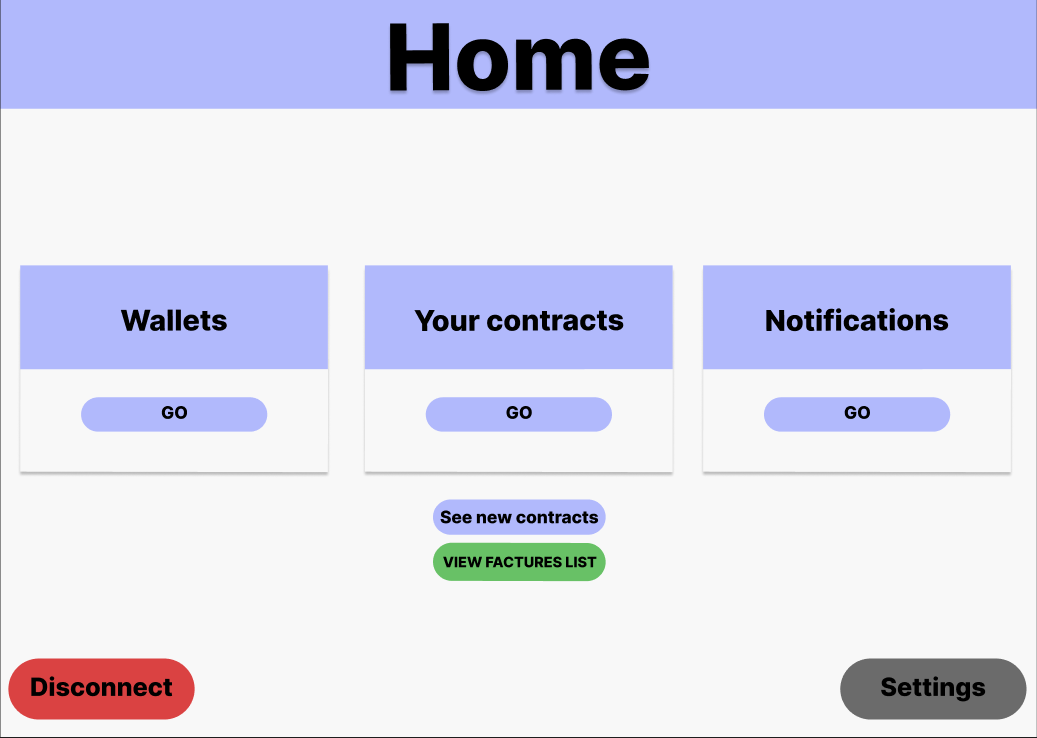
\includegraphics[width = 1\textwidth]{extension-maxime/interface/img/home.png}
\end{figure}

\subsection{Liste des factures}
\begin{flushleft}
Lorsque que le client a cliqué sur le bouton mentionné précédemment, celui-ci se retrouve face à sa liste des factures. L'interface contient donc la liste des factures payées et en attente de paiement. L'application affiche le numéro de la facture et le montant de l'acompte restant à payer.
\end{flushleft}
\begin{figure}[h]
\centering
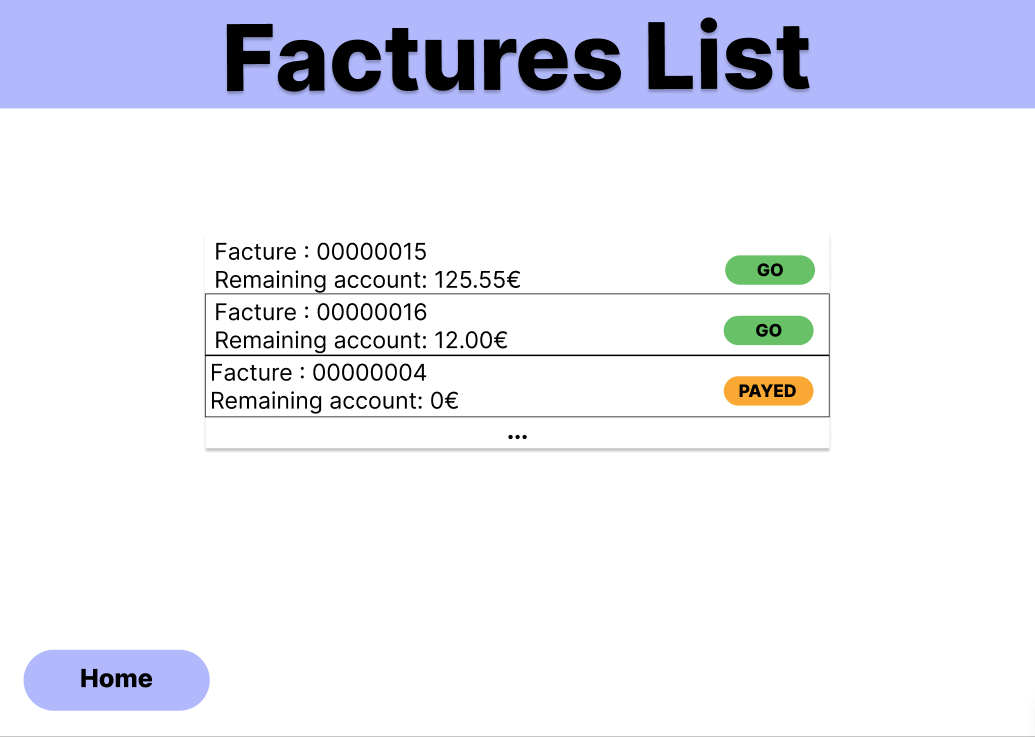
\includegraphics[width = 1\textwidth]{extension-maxime/interface/img/list.png}
\end{figure}

\subsection{Facture}
\begin{flushleft}
Lorsque que le client a accéder, via le menu précédent, à une facture, l'application affiche les détails correspondant à cette facture. Nous y retrouvons l'id du contrat associé, le montant annuel, le montant mensuel proposé/modifié, les informations de paiement, la méthode de paiement et son statut.
\end{flushleft}
\begin{figure}[h]
\centering
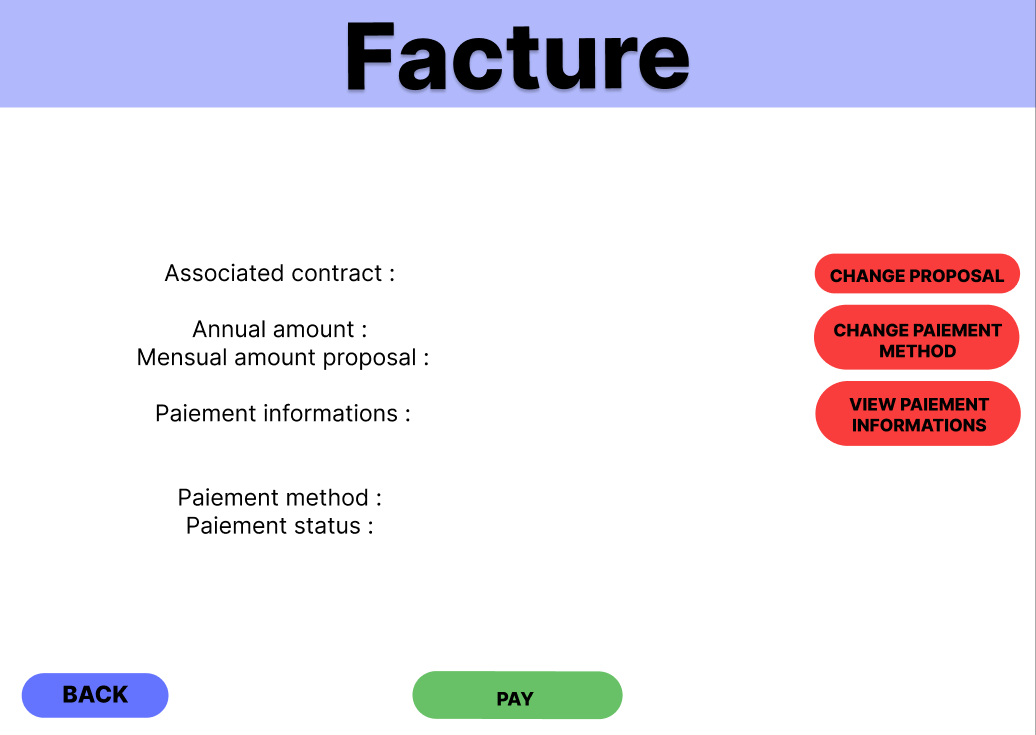
\includegraphics[width = 1\textwidth]{extension-maxime/interface/img/facture.png}
\end{figure}

\subsection{Paiement}
\begin{flushleft}
Si toutes les informations conviennent au client, celui-ci peut (dans le cas d'un paiement manuel) procéder au paiement où l'application affichera le QR Code correspondant au paiement.
\end{flushleft}
\begin{figure}[h]
\centering
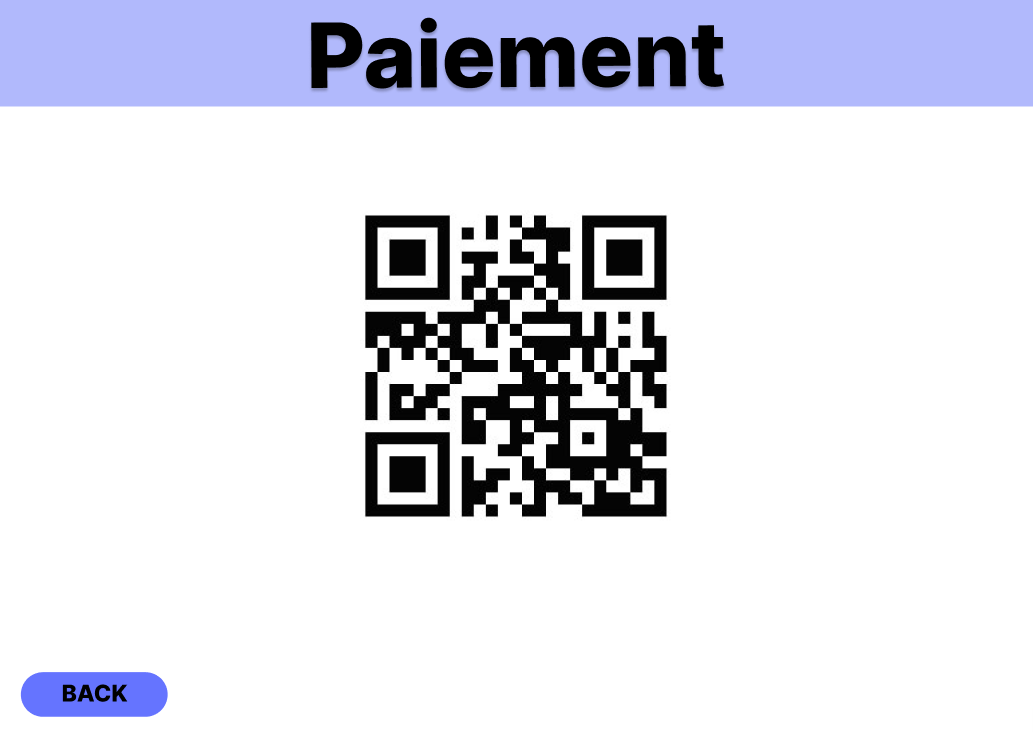
\includegraphics[width = 1\textwidth]{extension-maxime/interface/img/paiement.png}
\end{figure}

\subsection{Modification de la proposition}
\begin{flushleft}
Dans le cas où le client n'est pas satisfait de la proposition, celui-ci peut modifier la proposition en proposant un montant +- élevé. Une fois que le client clique sur le bouton "SUBMIT", celui-ci est renvoyé à la page précédente.
\end{flushleft}
\begin{figure}[h]
\centering
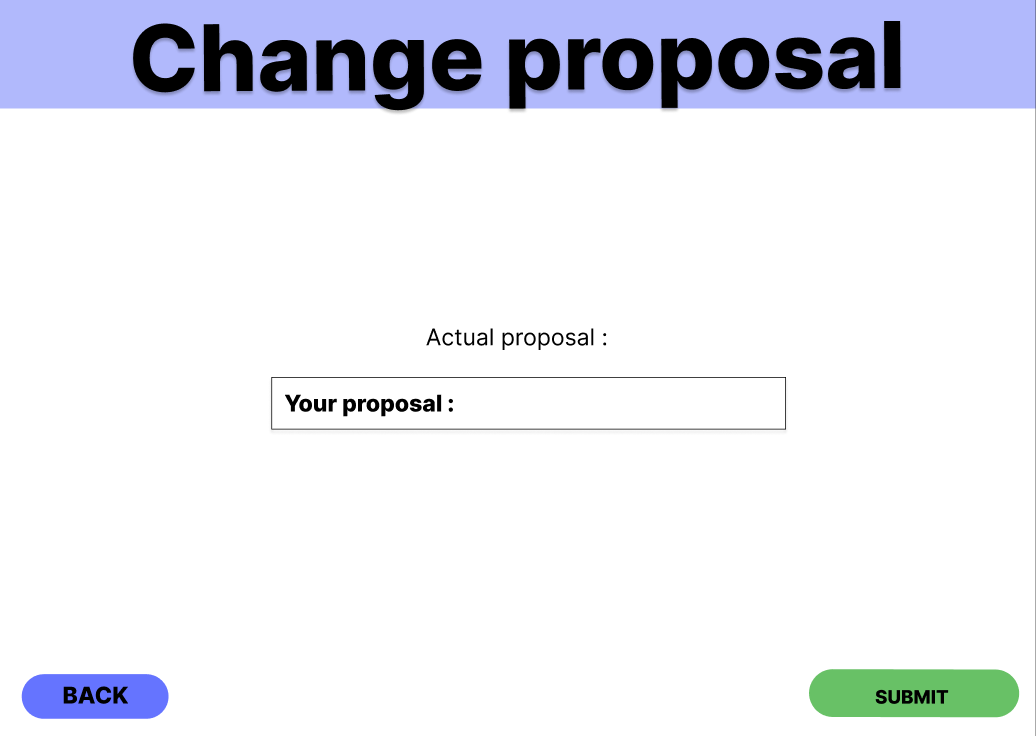
\includegraphics[width = 1\textwidth]{extension-maxime/interface/img/proposal.png}
\end{figure}

\subsection{Changement de méthode de paiement}
\begin{flushleft}
Si le mode de paiement ne convient pas au client, celui-ci peut le modifier et choisir entre mode "AUTOMATIC" ou "MANUAL" en cliquant sur les boutons correspondant. Une fois le choix fait, le client est ramené à la page précédente.
\end{flushleft}
\begin{figure}[h]
\centering
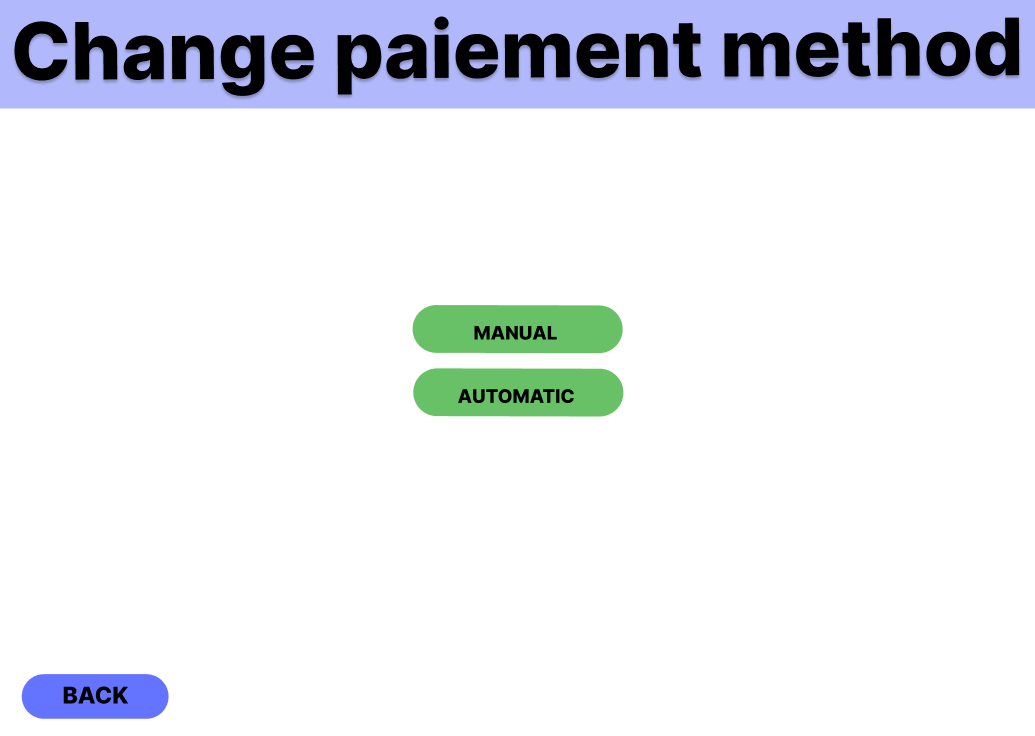
\includegraphics[width = 1\textwidth]{extension-maxime/interface/img/paiement-method.png}
\end{figure}

\subsection{Changement des informations bancaires}
\begin{flushleft}
Le client peut également voir ses informations bancaires et les modifier. L'applications affiche le nom du compte, son numéro, la date d'expiration ainsi que la date du prélèvement (dans le cas automatique). Ces informations peuvent être modifier en cliquant sur le bouton "CHANGE". La page est alors actualisée avec les nouvelles informations du client.
\end{flushleft}
\begin{figure}[h]
\centering
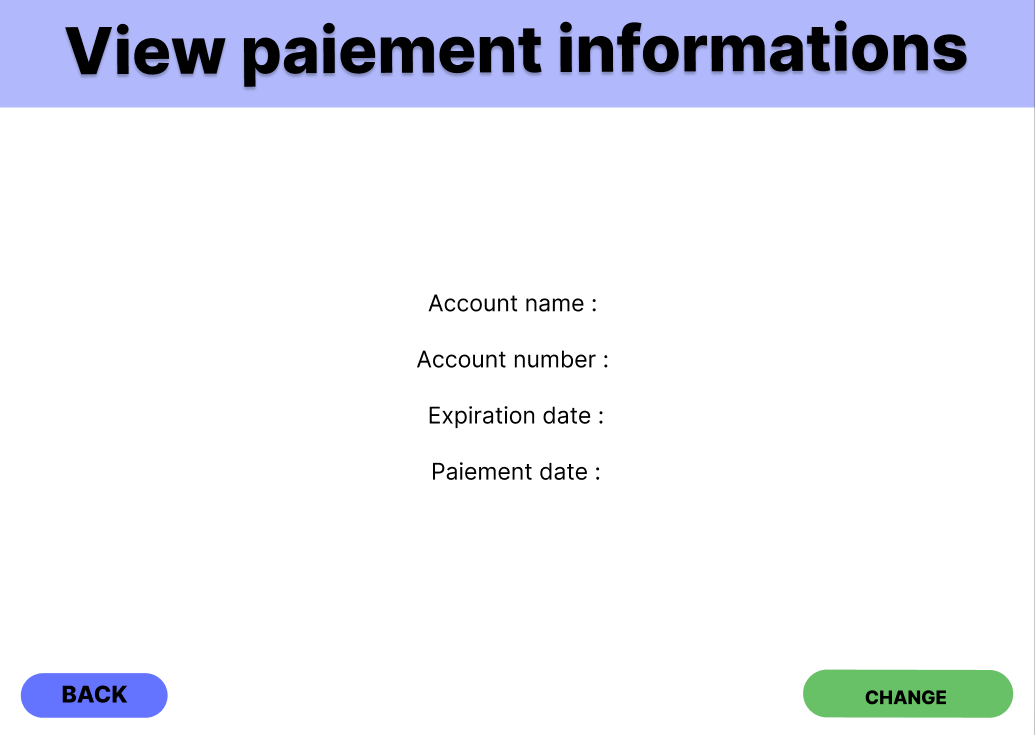
\includegraphics[width = 1\textwidth]{extension-maxime/interface/img/paiement-informations.png}
\end{figure}
